\chapter{RELATED WORK}
\label{relatedWorkChapter}
This thesis presents a visual analytics system to analyze risk and vulnerability based on the impacts to the international food trade network due to direct and cascading effects of a climate event. Current visualization tools in the area of climate change and the food trade network are examined. There are a number of relevant fields that are reviewed to understand these effects including the international food trade network, network graphs and visual analytics. Previous work on the topic of the food trade network, its composition and dependencies, is reviewed. As the food trade network is modeled as a network graph in this system, previous work on network graphs is reviewed. Lastly in order to present the system in an effective manner related work in the field of visual analytics is reviewed.\par

\section{Existing Visualizations}
A number of visualization systems have been developed to enable the exploration of food security, trade and climate change. I reviewed these systems and found a number of limitations related to this thesis. The general limitation of these systems is that the food trade network and food security indices are not modeled together and their interaction and analysis capabilities are limited in scope.\par
Climate change models and future food insecurity index forecasts are visualized on the \textit{Food Insecurity and Climate Change} website (Figure \ref{metOffice}), hosted by the Met Office and World Food Programme. The website allows users to explore different scenarios of adaptation to climate change and greenhouse gas emissions. The visualization presents a long range (2050s and 2080s) forecast of the potential for food insecurity based on these factors. However, the visualization does not consider the food trade network at all and does not allow for any simulation of specific climate events, preventing the use as a directed analysis tool.\par
\begin{figure}[htb]
	\center{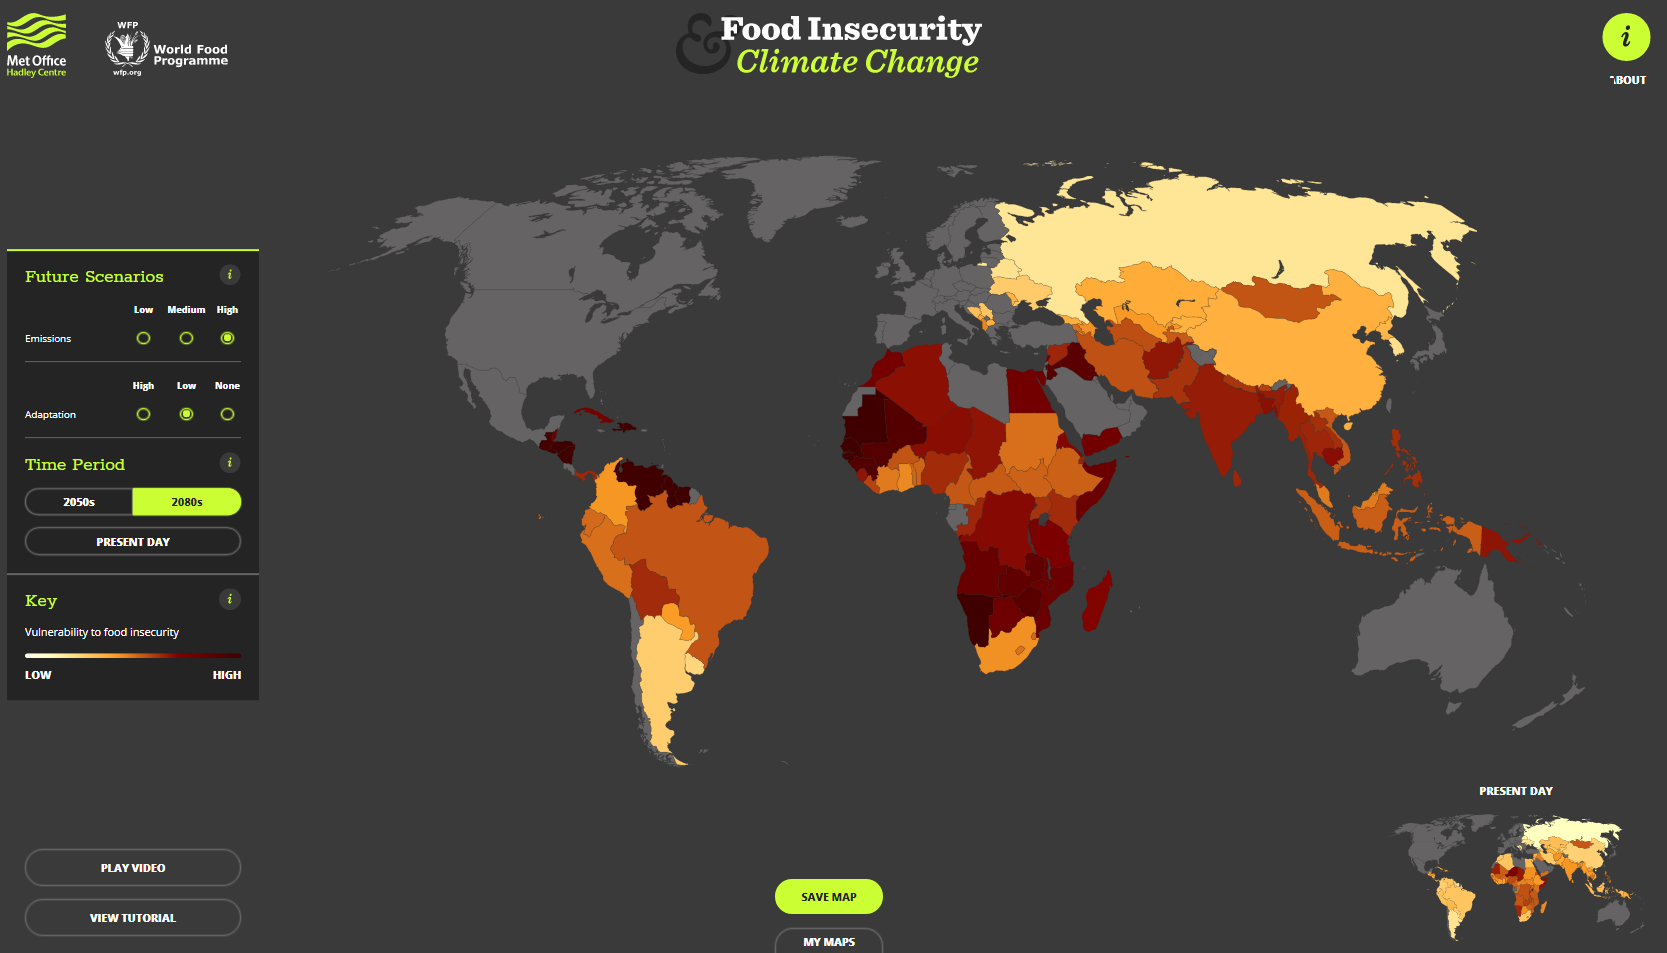
\includegraphics[width=\textwidth]{figures/metOffice.png}}
	\caption[MET OFFICE FOOD INSECURITY \& CLIMATE CHANGE WEBSITE]{Met Office Food Insecurity \& Climate Change website (www.metoffice.gov.uk/food-insecurity-index). The Met Office is the United Kingdom's national weather service. Their visualization shows a measure of how vulnerable a country's food security system is to the negative impacts of weather and climate \citep{metofficeCitation}. The darker red colors indicate a higher level of vulnerability. Future scenarios allow for predictions based on the options selected. The current display shows the vulnerability to food insecurity for the 2080s based on a scenario of high emissions and low adaptation levels.}
	\label{metOffice}
\end{figure}
Trade data can be visualized directly on the FAOSTAT website as seen in figure \ref{faostatViz}. This data visualization takes one country and displays the import or export trade links of a single trade good for that country. The visualization is done as a geographic choropleth representing the quantity or value of the imported or export good to another country. However, the visualization is ineffective as it only displays a single country's import or export contribution. It does not take into consideration the food trade network as a whole and does not allow for any interactions. These limitations again preclude any use for analyzing the effects of a change to the food trade network.\par
\begin{figure}[htb]
	\center{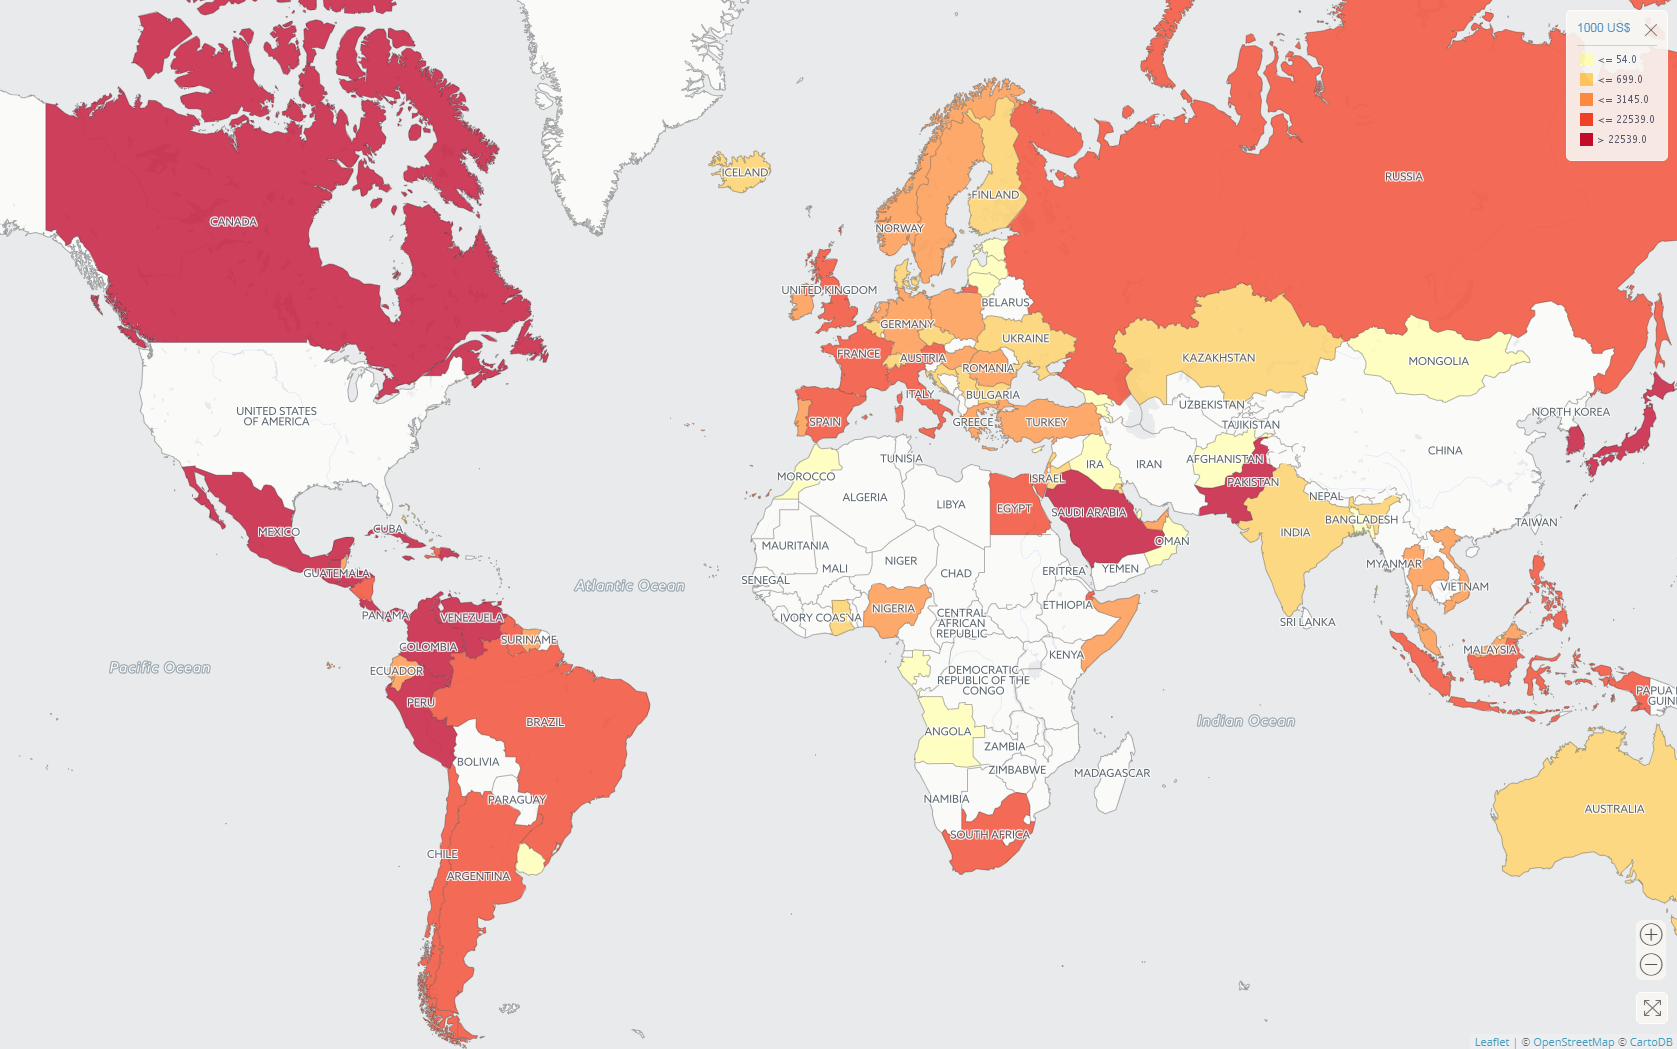
\includegraphics[width=\textwidth]{figures/faostatViz.png}}
	\caption[FAOSTAT DATA VISUALIZATION WEBSITE]{FAOSTAT data visualization website (www.fao.org/faostat/en/\#data/TM/visualize). The FAOSTAT is Food and Agriculture Organization of the United Nations Statistics Division. Their system shows the value of import or export trade links to or from the selected country for the given time period in a choropleth. The current display shows the dollar value of corn exported by the United States in the year 2013. The darker red the color a country is colored, the more the United States exported to that country. }
	\label{faostatViz}
\end{figure}

\section{Trade Networks and Food Security}
The increase of globalization has led to a marked decrease in the proportion of hungry people globally \citep{godfray2010food}. The international food trade network is used to feed people that were traditionally reliant on domestic production. Given that countries are becoming increasingly more import dependent \citep{d2014feeding}, the effects of disruptions to the food trade network are magnified. \cite{kali2007architecture} suggest that a network approach considering the cascading of shocks will be invaluable.\par
\cite{headey2011rethinking} highlights recent food crises and associates them to disruptions in the international food trade network due to surges in cereal prices. The cereal price surge in 2007 and 2008 is explored with an emphasis on how four staple good markets were negatively affected, leading to food security issues. Export restrictions and droughts were a major player in the volatility of the international food trade network at the time. According to \citep{brobakk2011increasing}, uncertainty in markets can lead to export bans which can lead to food insecurity. These works help provide understanding of the interaction between the trade network and food insecurity.\par
The food trade network can also be a tool to help deal with food security issues. Most of the global population is a resident of a net food importing country and so not self-sufficient, concluding that the world has moved from food insufficiency to an increasing food trade dependency \citep{porkka2013food}. This is especially true in the Middle East. The majority of Arabic countries import more than 50\% of their caloric intake \citep{faostat}. Suppliers are limited, with five exporters (Argentina, Australia, Canada, the European Union and the United States) accounting for almost three-quarters of the world's traded staple crops \citep{faostat}. \cite{d2016teleconnected} classifies countries vulnerability based on their level of caloric trade dependency. High dependency on a single staple crop for supply of calories and a high dependency on imports indicates a higher risk. This model of risk is used as the basis for the vulnerability index in this thesis.\par
Identified vulnerable countries also receive their imports from just a few dominant producing countries. \cite{silberglitt2015critical} explains the concern of two-tier pricing involved in concentrations of producers. Producers are able to influence the pricing on the market by enforcing export restrictions or bans, resulting in preferential domestic supplies. This has the potential of exacerbating the effects of a supply-side shock, which can be devastating to the entire food trade network. Exposure to non-domestic supply shocks is a trade-off to an increasingly globalized food trade network. According to \cite{gephart2016vulnerability}, exposure to this risk can be reduced by a diverse trade portfolio. These supply shocks are one representation of the cascading effects of a climate event.\par
An example of a supply shock by a major exporter is reviewed in \cite{fellmann2014harvest}. Russia, Ukraine and Kazakhstan temporarily placed export bans on wheat following poor harvest due to drought. This shows that shocks affecting more network-central countries are more likely to be transferred to other areas of the network. Net grain importing countries are at a major risk when diverse import trade portfolios are not present. This previous work provides the basis for my first case study.\par
The value of a link in the food trade network can be represented in many fashions. \cite{macdonald2015rethinking} suggest that in the modern era of globalization it may be more beneficial to think of a product's values using a resource metric such as cropland area. Monetary value can change with a number of factors and is so discouraged. Another useful metric we discovered may be calories or virtual water. Expanding on the concept of virtual water \cite{hoekstra2005globalisation} quantifies the calculations of water demand for specific crops. Virtual water balances are defined as the difference of gross virtual water imports and exports. Developed countries tend to have a more stable virtual water balance. Knowledge of the national virtual water balance is important in policy development because water scarcity is a driver of international food trade. \cite{konar2011water} explores the virtual water trade network as a amalgamation of the international food trade network. The topic provides a framework for use of water trade as the network model. Network graph statistics are produced for the virtual water representation of the international food trade network. Dominant countries are highly connected and are identified as hubs which connect to the large number of small trade-volume countries. \cite{hoekstra2012water} introduces water footprints and illustrates the global dimension of water consumption and pollution by showing that several countries heavily rely on foreign water resources. Many countries have significant impacts on water consumption and pollution elsewhere. Policies in this context translate to food security concerns and water footprints should be understood for development of these policies. This also solidifies the relationship between climate events, which generally affect water availability, and the food trade network. Because of increased globalization climate events are no longer localized and these regional events may have global effects on food security \citep{sternberg2012chinese}, validating the need for this second-order effect model.\par
Related work in the area of the international food trade network provides the preliminary domain-knowledge required for the effective development of a related visual analytic system. With understanding of the interactions and consequences of perturbations to the food trade network I was able to more effectively model the food trade network's cascaded effects. The literature reviewed here allowed for the connection between food insecurity vulnerability and the food trade network.\par







\section{Network Graphs}
To accurately model cascading effects we need to understand the topology of the international food trade network when represented as a node-edge graph. \cite{serrano2003topology} states the world trade network has become a self-organized complex system that must be considered in its entirety.\par
The international food trade network is essentially a very dense network graph and can be modeled as $G=(V,E,W,T)$. $V$ is the set of vertices, represented by all the countries involved in the food trade network. $E$ is the set of trade links, defined $E_n=\lbrace V_i, V_j, t \rbrace$. Direction is indicated with the importing country represented by $V_i \in V$ and the exporting country, $V_j \in V$. $T$ is the set of all trade goods. The good represented by an edge is $t \in T$. The weight of the edge is the defined as the function $w_{i,j,t}$. The weight function is the dollar value of the trade link of the specified good from country $j$ to $i$. The number of nodes is limited to the number of countries involved but the number of edges is extraordinary due to the large number of goods being traded and the number of unique trade partners.\par
Subgraphs are pieces of more complex networks and specifically three node subgraphs are labeled as triads. \cite{milo2002network} classifies these subgraphs occurring a significantly higher rates than expected as motifs. There are examples of motifs found in biological \citep{shen2002network}, technological \citep{milo2002network} and agricultural \citep{shutters2012agricultural} networks. The recurrence of these motifs show patterns that occur much more frequently in real networks than in randomized networks. This indicates that a structure exists which can be classified. A number of different classifications are presented and motif frequencies are examined for those distinct types. These network motifs are discovered here and also in \cite{grochow2007network}. This introduces a novel approach for motif discovery that utilizes a method for searching for a single network motif as opposed to enumerating subgraphs. It also takes advantage of symmetry of motifs to reduce the number of iterations. \cite{stouffer2012evolutionary} contains information on the different unique motif positions. This provides the reference when identifying the positions as well as the triad numerical classification. There are between one and three different unique motif positions depending on the type and thirty different unique positions over the thirteen different triads. The number and type of motifs in a network are important characteristics that directly affect stability of the network. The usefulness of using a reciprocal model for determination of the type of triad is confirmed in \cite{squartini2012triadic}. Models should take into account not only in the in and out degrees of the motifs but also the reciprocity of the links. With this representation the model can replicate the triadic structure. This suggests the dyadic structure of the network is information rich. \cite{zhou2016structure} employs a model that uses country behavior in the local triadic environment to account for the formation of such network structure. Different network graphs are created based on a country's top one or two trading partners. These truncated network graphs are shown to extract the more important information of the network. In this system these classifications of subgraphs are used to construct the triads.\par
Triad significance profiles (TSP) are an area of emerging research where the prevalence of certain triads is compared to normal distributions. \cite{winkler2013motifs} produces generative models that would create network graphs based on these triadic z-score profiles. \cite{shutters2012agricultural} lays the groundwork for association of triad significance profiles in the international food trade network to economic health. There are similarities of agricultural trade network with known triad significance profile of human social networks and biological information processing networks to a lesser degree. Superfamilies of existing networks are compared against the international food trade network and a distinct superfamily for the food trade network is identified. My framework visualizes these TSP for potential association to food trade network health.\par
Other related works focus on the international food trade network's specific network graph statistics \cite{fagiolo2010evolution} and topology \citep{serrano2003topology}. The density of the network graph as indicated by \cite{schiavo2010international} shows that there is a high level of clustering and that the topology of the international trade network is indeed important. Three data points for nodes are defined; node degree (the number of links maintained by each node), average nearest neighbor degree (the correlation between the degree of a node and the average degree of its partners) and clustering coefficient (the percentage of pairs of a node's partners that are connected among themselves). Importance should be given to the distribution of trade links across all trade partners. \cite{kali2007architecture} explains that a country's position in the network has substantial implications for quantifying economic growth. The majority of countries involved in the trade network are characterized by weak links, with a small number of countries exhibiting strong relationships indicating a core-periphery structure. The clustering coefficient is high in the international food trade network and has a high level of centralization, implying a hierarchical structure as suggested in other research (\cite{zhou2016structure}, \cite{garlaschelli2005structure}). \cite{zhou2016structure} constructs the network based on the top trade links and indicates there is indeed a hierarchy. \citep{ravasz2003hierarchical} and \citep{zhou2016structure} show that real networks are not randomized, but follow a pattern of organization related to hierarchy. At higher levels of trade, the network is considered scale-free; there is no typical country in terms of number of trading partners. The properties of scale-free networks are examined in \cite{li2005towards}. The power law degree distributions of the international food trade network align with these observations.\par
As the international food trade network was modeled as a network graph, the literature reviewed here allowed for an effective understanding of the underlying construction. The dependencies in the food trade network are related to the topology of the network graph. Although TSP analysis was passed in favor of a cascading effect model the foundation for future work is established with the related work here.\par


\section{Visual Analytics}
Visual analytics has become the preferred tool for domain-experts exploring large data sets. It is defined by \cite{cook2005illuminating} as ``analytical reasoning facilitated by interactive visual interfaces.'' \cite{shneiderman1996eyes} introduces the well-known information seeking mantra: overview first, zoom and filter, then details-on-demand. Visual analytics, per \cite{keim2006challenges}, extends this mantra to include the combination of data analysis and interactive visual interfaces: ``analyze first, show the important, zoom/filter/analyze further and details on demand.''\par
	\begin{figure}[htb]
		\center{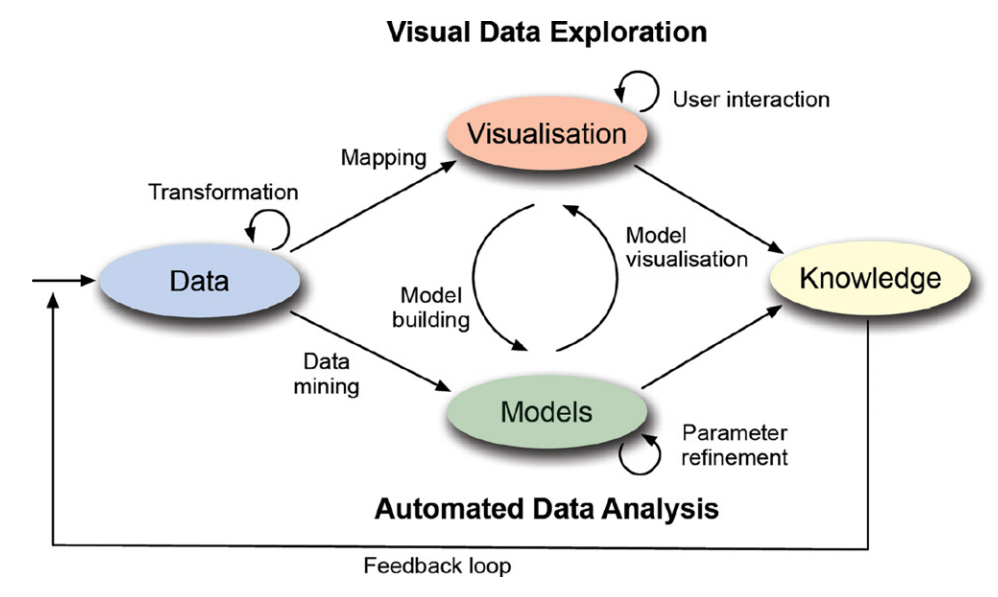
\includegraphics[width=\textwidth]{figures/keim.png}}
		\caption[VISUAL ANALYTICS FRAMEWORK]{Visual Analytics Framework, (\cite{keim2008visual}, \cite{kohlhammer2011solving})}
		\label{keim}
	\end{figure}
\cite{keim2008visual} introduces the framework for visual analytics (Figure \ref{keim}). The framework captures the process of a typical sense-making session. First, data is transformed by filtering and models are built from the resultant data subset. Visual data exploration is then applied with interactive visualizations to analyze and explore the data. Automatic analysis is done at each iteration of a feedback loop to produce results. The feedback loop helps repeat this process until sufficient refinement of the results is achieved. This automated analysis techniques were used by this thesis to calculate vulnerability indices after each iteration of the feedback loop.\par
To build the visual analytics system, the first step is data analysis. Previous research (\cite{zhou2016structure}, \cite{shutters2012agricultural}, \cite{squartini2012triadic}) has provided some initial data analysis that is supplemented by our own resources. Triads are calculated, motif positions are generated and bilateral trade links are computed. Further analysis is accomplished by the user interaction and filtering of interesting data in the feedback loop.\par
The next step is analysis via interactions with the visualizations. In visual analytics involving graphs, \cite{sun2013survey} shows recent research has focused on the visual mapping aspect of the analytics systems over the model-based analysis. Graph data is highly structured and is a possible reason for this paradigm.\par
Visualizing a network graph can be done in two primary ways: node-link diagrams and adjacency matrices. The most familiar visualization is the node-link diagram . \cite{ghoniem2004comparison} considers the two different representation and compares the readability of the two graphs. Although the international trade network starts out with a large number of nodes, when filtering is applied \citep{shneiderman1996eyes} it has a limited number of nodes. Therefore when choosing the appropriate visualization I consider it a small graph, and node-link diagrams are more readable \citep{ghoniem2004comparison}.\par
Node placement is a consideration when network visualization is concerned. A common layout strategy is based on geographic representation \citep{shneiderman2006network}. This geographically representative positioning is used in both of the main visual representations. The linked multiple views of the familiar world map (choropleth) and the network visualization allow for a greater understanding \citep{rodgers2005graph} and allow for mental mapping \citep{eades1991preserving}.\par
When visualizing a network minimizing edge crossing is the most important aesthetic consideration \citep{purchase1997aesthetic} for improving human comprehension. A number of different algorithms for graph visualization were reviewed (\cite{herman2000graph}, \cite{dunne2013motif}, \cite{holten2009force}) that help with this consideration. \cite{herman2000graph} overviews a number of basic graph layout algorithms in the context of information visualization. \cite{dunne2013motif} offers a technique to simplify highly clustered network graphs by aggregating subnetworks. Simplifying the drawing of certain types of motifs can greatly increase readability in dense network graphs. \cite{holten2009force} shows another example of a technique aimed at simplifying complex network graphs. This is achieved by bundling of similarly drawn edges and subsequent splitting of the edges closer to the termination node. Ultimately these algorithms were removed from consideration in favor of mental mapping \citep{eades1991preserving} and interpretability \citep{keim2008visual}. Nodes were positioned approximately geographic to aid in the establishment of this mental map. The minimization of edge crossing is accomplished interactively by dragging of nodes after a simulation baseline is established.\par
The parameters for the algorithms are usually considered in multiple solutions before results are achieved \citep{hund2016visual}. In this system the reasoning is done by the human analyst \citep{andrienko2011challenging}, and the interaction allows for the parameters of the algorithms to be manipulated by the users.\par
Knowledge in this field was pertinent to the development of effective human computer interaction techniques used in this system. The visual analytic paradigm providing for the feedback loop was implemented to allow for analysis of the effects of a simulated climate event.\par
The work reviewed here provides the framework for my visual analytic system. I build the framework on the principles defined in the visual analytics mantra \citep{keim2006challenges}. The representation of the network graph as a node-link diagram instead of an adjacency matrix was based on the suggestions of previous research included in this section. The visual design was also inspired by the mental mapping paradigm.\par